%%%%%%%%%%%%%%%%%%%%%%%%%%%%%%%%%%%%%%%%%%%%%%%%%%%%%%%%%%%%%%%%%%%%%%%%%%%%%%%%
% Template for USENIX papers.
%
% History:
%
% - TEMPLATE for Usenix papers, specifically to meet requirements of
%   USENIX '05. originally a template for producing IEEE-format
%   articles using LaTeX. written by Matthew Ward, CS Department,
%   Worcester Polytechnic Institute. adapted by David Beazley for his
%   excellent SWIG paper in Proceedings, Tcl 96. turned into a
%   smartass generic template by De Clarke, with thanks to both the
%   above pioneers. Use at your own risk. Complaints to /dev/null.
%   Make it two column with no page numbering, default is 10 point.
%
% - Munged by Fred Douglis <douglis@research.att.com> 10/97 to
%   separate the .sty file from the LaTeX source template, so that
%   people can more easily include the .sty file into an existing
%   document. Also changed to more closely follow the style guidelines
%   as represented by the Word sample file.
%
% - Note that since 2010, USENIX does not require endnotes. If you
%   want foot of page notes, don't include the endnotes package in the
%   usepackage command, below.
% - This version uses the latex2e styles, not the very ancient 2.09
%   stuff.
%
% - Updated July 2018: Text block size changed from 6.5" to 7"
%
% - Updated Dec 2018 for ATC'19:
%
%   * Revised text to pass HotCRP's auto-formatting check, with
%     hotcrp.settings.submission_form.body_font_size=10pt, and
%     hotcrp.settings.submission_form.line_height=12pt
%
%   * Switched from \endnote-s to \footnote-s to match Usenix's policy.
%
%   * \section* => \begin{abstract} ... \end{abstract}
%
%   * Make template self-contained in terms of bibtex entires, to allow
%     this file to be compiled. (And changing refs style to 'plain'.)
%
%   * Make template self-contained in terms of figures, to
%     allow this file to be compiled. 
%
%   * Added packages for hyperref, embedding fonts, and improving
%     appearance.
%   
%   * Removed outdated text.
%
%%%%%%%%%%%%%%%%%%%%%%%%%%%%%%%%%%%%%%%%%%%%%%%%%%%%%%%%%%%%%%%%%%%%%%%%%%%%%%%%

\documentclass[letterpaper,twocolumn,10pt]{article}
\usepackage{usenix2019_v3}

% to be able to draw some self-contained figs
\usepackage{tikz}
\usepackage{amsmath}

% inlined bib file
\usepackage{filecontents}

%-------------------------------------------------------------------------------
\begin{filecontents}{\jobname.bib}
%-------------------------------------------------------------------------------
@Book{arpachiDusseau18:osbook,
  author =       {Arpaci-Dusseau, Remzi H. and Arpaci-Dusseau Andrea C.},
  title =        {Operating Systems: Three Easy Pieces},
  publisher =    {Arpaci-Dusseau Books, LLC},
  year =         2015,
  edition =      {1.00},
  note =         {\url{http://pages.cs.wisc.edu/~remzi/OSTEP/}}
}
@InProceedings{waldspurger02,
  author =       {Waldspurger, Carl A.},
  title =        {Memory resource management in {VMware ESX} server},
  booktitle =    {USENIX Symposium on Operating System Design and
                  Implementation (OSDI)},
  year =         2002,
  pages =        {181--194},
  note =         {\url{https://www.usenix.org/legacy/event/osdi02/tech/waldspurger/waldspurger.pdf}}}
\end{filecontents}

%-------------------------------------------------------------------------------
\begin{document}
%-------------------------------------------------------------------------------

%don't want date printed
\date{}

% make title bold and 14 pt font (Latex default is non-bold, 16 pt)
\title{\Large \bf CS131 Homework 3 Report}

%for single author (just remove % characters)
\author{
{\rm Melody Chen}\\
Discussion 1C
% copy the following lines to add more authors
% \and
% {\rm Name}\\
%Name Institution
} % end author

\maketitle


%-------------------------------------------------------------------------------
\section{Introduction}
%-------------------------------------------------------------------------------

In this homework assignment, we focus on the programming language, Java, and Java synchronization, which is based on the Java Memory Model (JMM). JMM defines how an application can safely avoid data races when accessing shared memory. It allows our Java program to optimize accesses by using different threads interleave in a schedule that assumes sequential consistency. For this homework, we are tasked with comparing performances of different implementations of long array when the program is multi-threaded. According to Doug Lea's "Using JDK 9 Memory Order Modes", multi-threaded programs that are performed on multi-core processors that are not carefully written often lead to race conditions due to two threads being executed without a pre-determined order where neither precedes the other, memory operations across different processors may not be executed atomically, and the fact that CPUs process instructions in an overlapped fashion. In the rest of the report, we explore in detail how to prevent race conditions and the performance of different methods to prevent race condition in Java in addition to evaluating their performances of varying platforms.


\section{Statistics about Testing Platform}
%-------------------------------------------------------------------------------

The two testing platforms I chose were \texttt{lnxsrv06} and \texttt{lnxsrv09}. I chose these two platforms as they have differing CPU types, which will allow us to make meaningful comparisons later on. \texttt{lnxsrv09} has cpu model that is "Intel(R) Xeon(R) CPU E5-2640 v2 @ 2.00GHz in contrast to \texttt{lnxsrv06} which has cpu model that is "Intel(R) Xeon(R) CPU E5620  @ 2.40GHz". Thus, cpu on \texttt{lnxsrv06} is slightly faster than cpu of \texttt{lnxsrv09}. Aside from the cpu model, \texttt{lnxsrv09} has 31 processors in contrast to \texttt{lnxsrv06} which only has 15 processors. The more processors you have the more threads you can run at once, thus the number of processors may affect our results shown later. Comparing the meminfo of the two servers, we can see that the total memory size is very similar, but the total free memory differs in that \texttt{lnxsrv09} has significantly more free memory than \texttt{lnxsrv06}. The more free memory available means more memory can be cached which increases access speed, which can increase the speed of our running program. The output of \texttt{java -version} is the same for the two platforms, with the following output:
\begin{verbatim}
java 13.0.2 2020-01-14
Java(TM) SE Runtime Environment (build 13.0.2+8)
Java HotSpot(TM) 64-Bit Server VM 
(build 13.0.2+8, mixed mode, sharing)
\end{verbatim}
Thus, the two versions of java we're using to compile and run our program is the same.

\section{AcmeSafeState Implementation}
For my implementation of AcmeSafeState, I chose to use the \texttt{java.util.concurrent.atomic} package in order to have a safe multi-threaded program that has critical sections that are protected and implemented as atomic instructions. Unlike the synchronized implementation of long array, we do not use locks which corresponds to built in \texttt{synchronized} blocks in Java, which is described in detail in Lea's paper. The \texttt{java.util.concurrent.atomic} package include methods corresponding to the VarHandle constructions also mentioned in Lea's paper. We do not need to use VarHandles in our RCF(Race Condition Free) implementation of AcmeSafeState as it is part of the \texttt{java.util.concurrent.atomic} package. Within this package, it has classes that do many array-related operations atomically, and thus prevents the scheduler and other threads from interfering with the operation and cause race conditions. The problem with our unsynchronized implementation of long array was that too many threads are trying to change the values of the long array at the same time, which is characterized in Lea's paper as "Task Parallelism, Memory Parallelism, and Instruction Parallelism", and the scheduler could switch out certain threads in the middle of their operations, causing many increments and decrements to be incomplete. Now through the use of \texttt{java.util.concurrent.atomic} package, we have access to a class, "AtomicLongArray", that has atomic instructions that we can use to do the increment and decrement operations. No longer will we have the problem of the unsynchronized implementation, as every operation we do in AcmeSafeState is atomic and cannot therefore be interrupted. These instructions will either be executed fully or not be counted as executed. Thus, we are free to run our multi-threaded program with the AcmeSafeState and receive Race Condition Free results.

\section{Problems Faced}
One of the problems I faced in order to do my measurements of the performance of different classes accurately was encountered when I was writing my AcmeSafeState class. As I have not coded in Java for a while, I had trouble importing the \texttt{java.util.concurrent.atomic} package in order to use the class AtomicLongArray. But once, I looked at the documentations provided by the specs, I was able to understand how to import packages correctly into my Java program. \par
Another problem I faced was when I was trying to obtain the data of running the program with different classes, different number of values, and different number of threads. It looked like manually running everything on both of my platforms, through commands in the \texttt{lnxsrv}s, would take a long time. So I decided to write a bash script to solve this problem.

%---------------------------
\begin{figure}
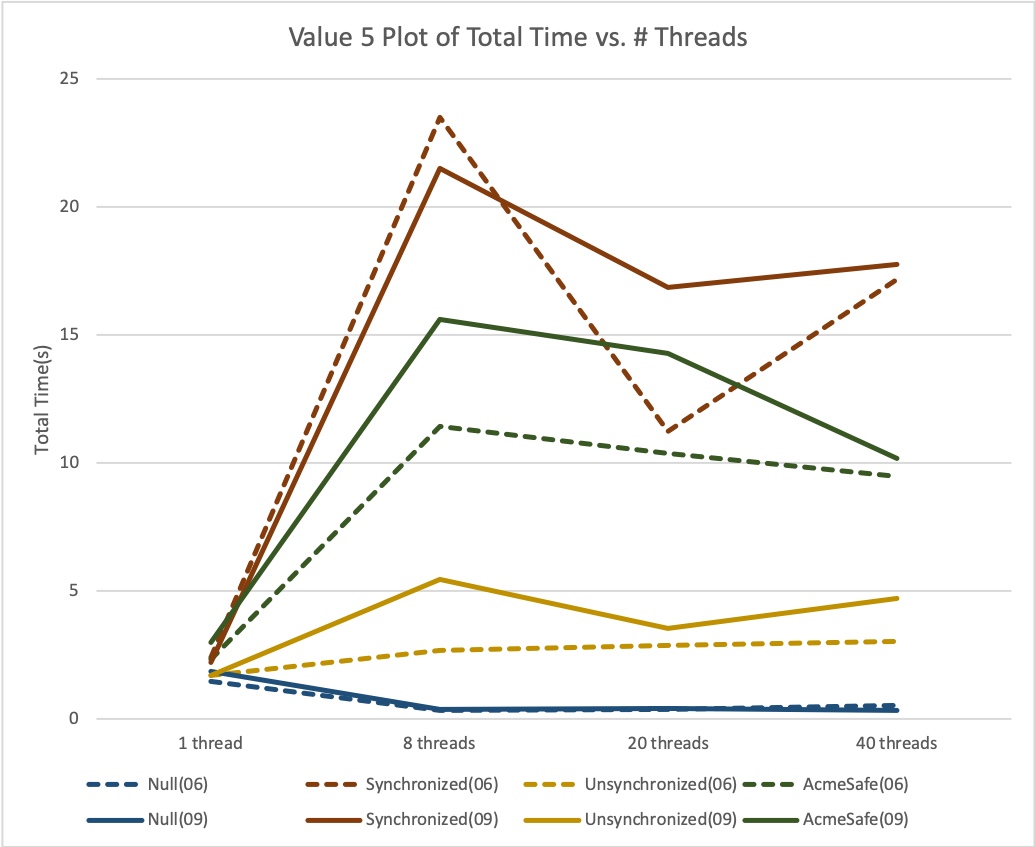
\includegraphics[scale=0.45]{totaltime-value5.png}
\caption{\label{fig:vectors} Plot of Measurement(Total Time) of Performance of SwapTest on Long Array for 5 values with 100000000 transitions. Dash lines imply that measurement is from \texttt{lnxsrv06} and solid lines imply that measurement is from \texttt{lnxsrv09.} }
\end{figure}
%% %---------------------------
%---------------------------
\begin{figure}
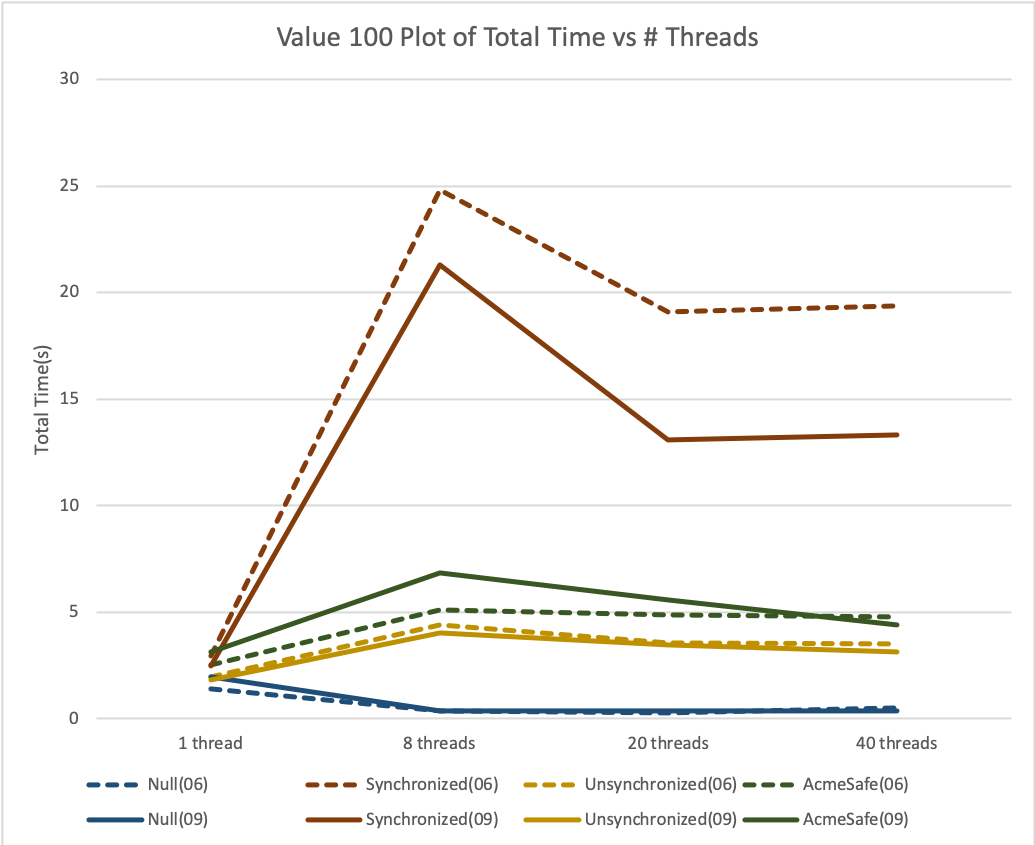
\includegraphics[scale=0.45]{totaltime-value100.png}
\caption{\label{fig:vectors} Plot of Measurement(Total Time) of Performance of SwapTest on Long Array for 100 values with 100000000 transitions. Dash lines imply that measurement is from \texttt{lnxsrv06} and solid lines imply that measurement is from \texttt{lnxsrv09.} }
\end{figure}
%% %---------------------------
%---------------------------
\begin{figure}
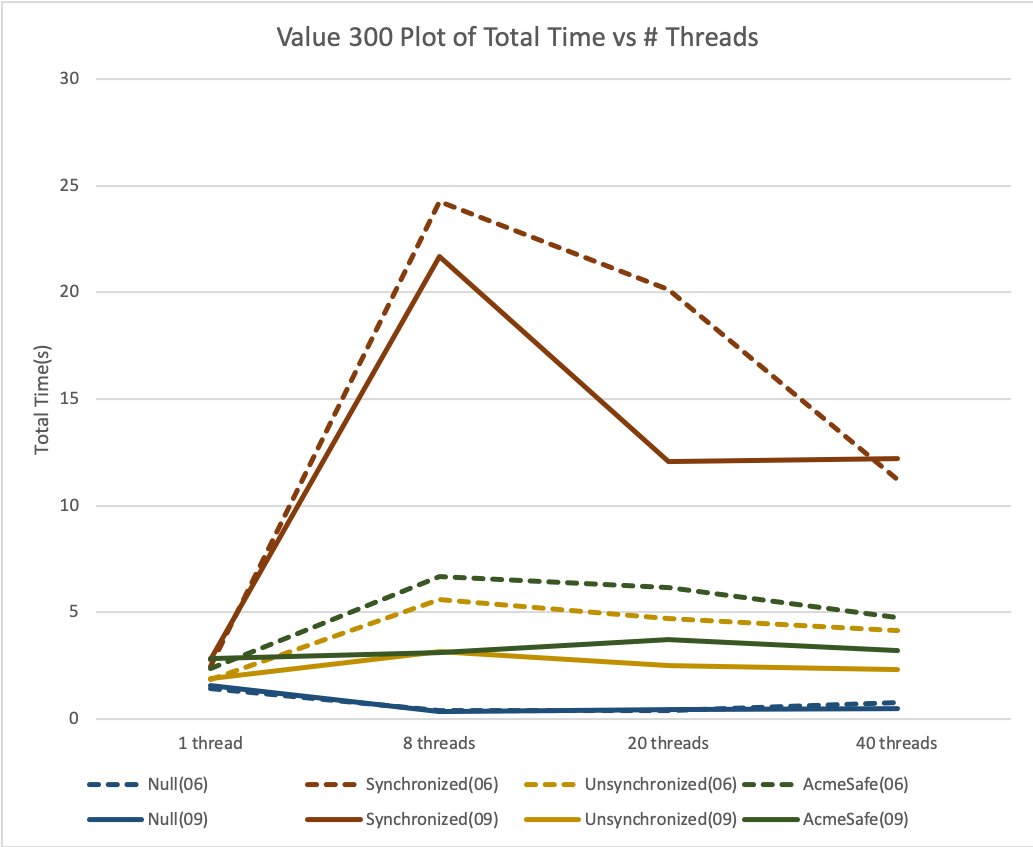
\includegraphics[scale=0.45]{totaltime-value300.png}
\caption{\label{fig:vectors} Plot of Measurement(Total Time) of Performance of SwapTest on Long Array for 300 values with 100000000 transitions. Dash lines imply that measurement is from \texttt{lnxsrv06} and solid lines imply that measurement is from \texttt{lnxsrv09.} }
\end{figure}
%% %---------------------------

\section{Measurement and Analysis}
The class \texttt{unsafeMemory.java} allows us to run SwapTest on our different implementations of the interface \texttt{state}. The result are measurements of the total real time and CPU time in seconds of our SwapTest and average real swap time and average CPU swap time in nanoseconds. The measurement I choose to focus on for analysis is total real time. From the data outputted by \texttt{unsafeMemory.java}, we can see that although CPU time differs from real time, they have strong correlation, so we choose to focus on total real time to not overwhelm the reader with data points. We also choose to focus on real average swap time for one of the graphs as it gives a clear image of how much time each swap takes, averaging out the overhead based on the number of threads and transitions. \par
From Figure 1, 2, and 3, we can see that for a long array of 5 values, the synchronized implementation is overall the slowest, and the AcmeSafeState implementation is the second slowest. AcmeSafeState is expected to run faster than SynchronizedState as AcmeSafeState uses atomic functions to prevent race conditions, which is faster than using the naive method of synchronized key word to lock the entire function. As expected, the null implementation runs the fastest as the swap function does not do anything. The unsynchronized version is the second fastest as it does not try to prevent race condition from occurring, which leads to running UnsynchronizedState leading to errors if the number of threads is greater than 1. \par
We can also see from these figures that for one thread, all four implementations have around the same speed as with one thread there will be no thread contentions and no risk of data races, so there is no need to wait for other threads which is what causes the bigger time gap for SynchronizedState later on. AcmeSafeState is the slowest for 1 thread as regardless of whether there are multiple threads contending or just one thread, it does the same atomic operation, which is slower than regular implementations of increment and decrement. \par 
From Figure 1, we cannot see clearly the effect of running the same program on two different servers. But, from Figure 2 and 3, we can observe that for the majority of the time \texttt{lnxsrv06} runs slower than \texttt{lnxsrv09}, which makes sense as \texttt{lnxsrv09} has many more processors and free memory than \texttt{lnxsrv06}. The more processors you have, the more threads you can run simultaneously, which decreases the total time of your program. Occasionally, we see that \texttt{lnxsrv06} runs faster than \texttt{lnxsrv09}, and this could be due to \texttt{lnxsrv06} having a slightly faster CPU than \texttt{lnxsrv09}. Slight variations may also be due to many other programs being run on the servers at the same time by other users. \par
In Figure 4, we focus on the average real swap time instead of total time in order to see how the number of threads, type of implementations, and platform affect the duration of each swap. From Figure 4, we can clearly observe that \texttt{lnxsrv06} is slower than \texttt{lnxsrv09} for each swap operation, which is mainly due to the significantly more number of processors and free memory that is available in \texttt{lnxsrv09}. We can also clearly observe that with more number of threads the average swap time increases, and this is likely due to the fact that the higher the number of threads, the more threads that are contending to be scheduled by the scheduler, which could lead to overhead that increases the average swap time. Similar to what we concluded in previous paragraphs, it is clear from Figure 4 that SynchronizedState is significantly slower than our AcmeSafeState, which shows that our implementation of AcmeSafeState which does not output any errors for all the tests ran, achieves better performance than SynchronizedState while retaining safety!

%---------------------------
\begin{figure}
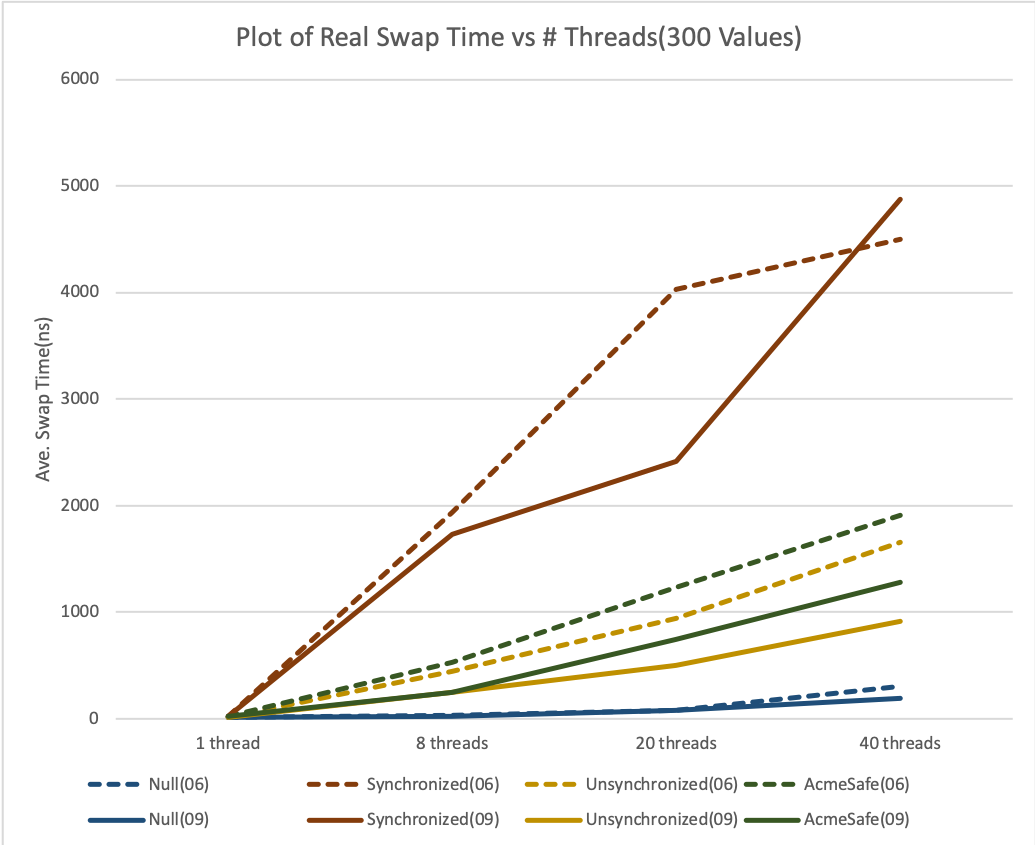
\includegraphics[scale=0.45]{swaptime-value300.png}
\caption{\label{fig:vectors} Plot of Measurement(Ave. Swap Time) of Performance of SwapTest on Long Array for 300 values with 100000000 transitions. Dash lines imply that measurement is from \texttt{lnxsrv06} and solid lines imply that measurement is from \texttt{lnxsrv09.} }
\end{figure}
%% %---------------------------


\section*{Acknowledgments}
%-------------------------------------------------------------------------------

Thank you to Professor Eggert and the TAs for introducing and grading our homeworks.

%-------------------------------------------------------------------------------

%-------------------------------------------------------------------------------
\bibliographystyle{plain}
\bibliography{\jobname}
Lea's Paper \\
http://gee.cs.oswego.edu/dl/html/j9mm.html \\
AtomicLongArray Documentation \\ https://docs.oracle.com/en/java/javase/13/docs/api/java.base/java/ \\ util/concurrent/atomic/AtomicLongArray.html \\
Project Specifications \\ https://web.cs.ucla.edu/classes/spring20/cs131/hw/hw3.html
%%%%%%%%%%%%%%%%%%%%%%%%%%%%%%%%%%%%%%%%%%%%%%%%%%%%%%%%%%%%%%%%%%%%%%%%%%%%%%%%
\end{document}
%%%%%%%%%%%%%%%%%%%%%%%%%%%%%%%%%%%%%%%%%%%%%%%%%%%%%%%%%%%%%%%%%%%%%%%%%%%%%%%%

%%  LocalWords:  endnotes includegraphics fread ptr nobj noindent
%%  LocalWords:  pdflatex acks